\documentclass[aspectratio=169]{beamer}

% Document metadata
\title{git-annex : a short introduction}
\subtitle{Pierre-Antoine Senger}
\institute{University of Strasbourg}
\date{\today}

% Image for the title page (use includegraphics option to properly size/place it)
\titlegraphic{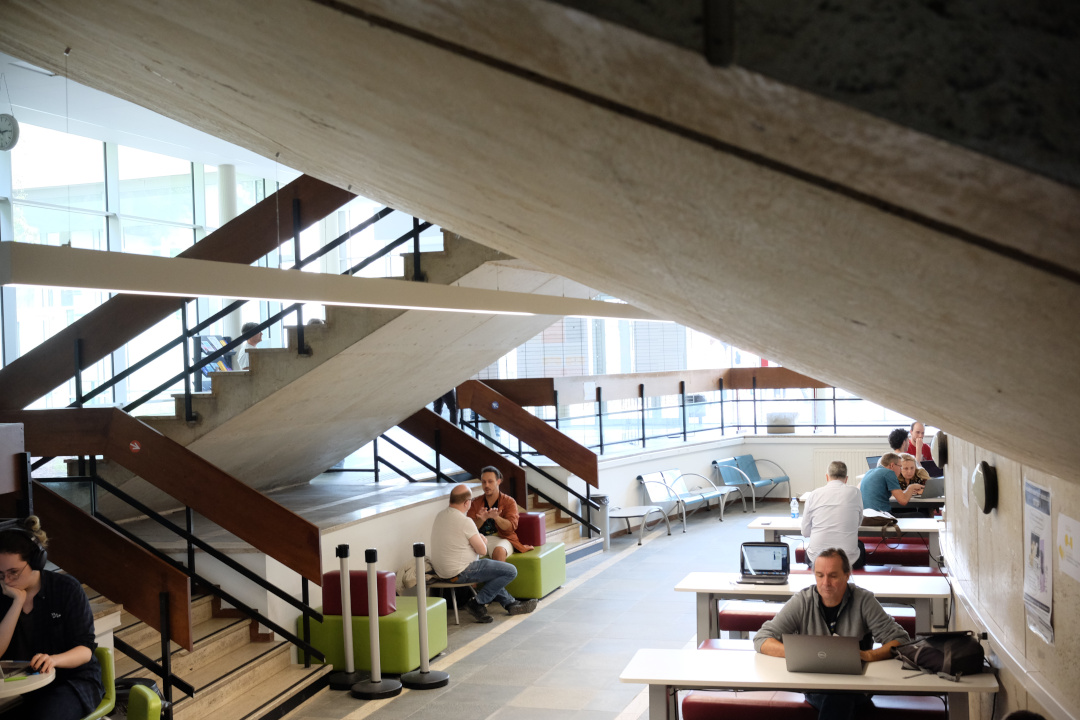
\includegraphics[height=\paperheight]{math-info.jpg}}

\usetheme[sectionstyle=style2]{trigon}

% Define logos to use (comment if no logo)
\biglogo{logo-ufr.png} % Used on titlepage only
\smalllogo{trigon_small.pdf} % Used on top right corner of regular frames

% ------ If you want to change the theme default colors, do it here ------
%\definecolor{tPrim}{HTML}{00843B}   % Green
%\definecolor{tSec}{HTML}{289B38}    % Green light
%\definecolor{tAccent}{HTML}{F07F3C} % Orange

% ------ Packages and definitions used for this demo. Can be removed ------
\usepackage{appendixnumberbeamer} % To use \appendix command
\pdfstringdefDisableCommands{% Fix hyperref translate warning with \appendix
  \def\translate#1{#1}%
}
\usepackage{pgf-pie} % For pie charts
\usepackage{caption} % For subfigures
\usepackage{subcaption} % For subfigures
\usepackage{xspace}
\newcommand{\themename}{\textbf{\textsc{trigon}}\xspace}
\usepackage[scale=2]{ccicons} % Icons for CC-BY-SA
\usepackage{booktabs} % Better tables
\usepackage{amsmath, amsfonts}
\usepackage[T1]{fontenc}
\usepackage[utf8]{inputenc}
\usepackage{graphicx}
\usepackage{pgfplots}
\usepackage{siunitx}
\usepackage{bm}
\usepackage{algorithm}
\usepackage{algpseudocode}
\usepackage{listings}
\usetikzlibrary{arrows.meta, shapes, snakes}
\pgfplotsset{compat=1.18}
\usepackage[backend=biber,style=alphabetic]{biblatex} % Bibliography management
\addbibresource{references.bib}
\graphicspath{{images/}}

%==============================================================================
%                               BEGIN DOCUMENT
%==============================================================================
\begin{document}

%--------------------------------------
% Create title frame
\titleframe

%--------------------------------------
% Table of contents
\begin{frame}{Overview}
  \setbeamertemplate{section in toc}[sections numbered]
  \tableofcontents[hideallsubsections]
\end{frame}

%--------------------------------------
\section{Context}
\begin{frame}{Context}
  \begin{itemize}
    \item \textbf{HPC} often requires large datasets (meshes, post-processing data, etc.).
    \item \textbf{Git} is not designed for large files and gets very slow.
  \end{itemize}
  %   \vspace{0.5em}
  \begin{center}
    \begin{minipage}{0.49\textwidth}
      \centering
      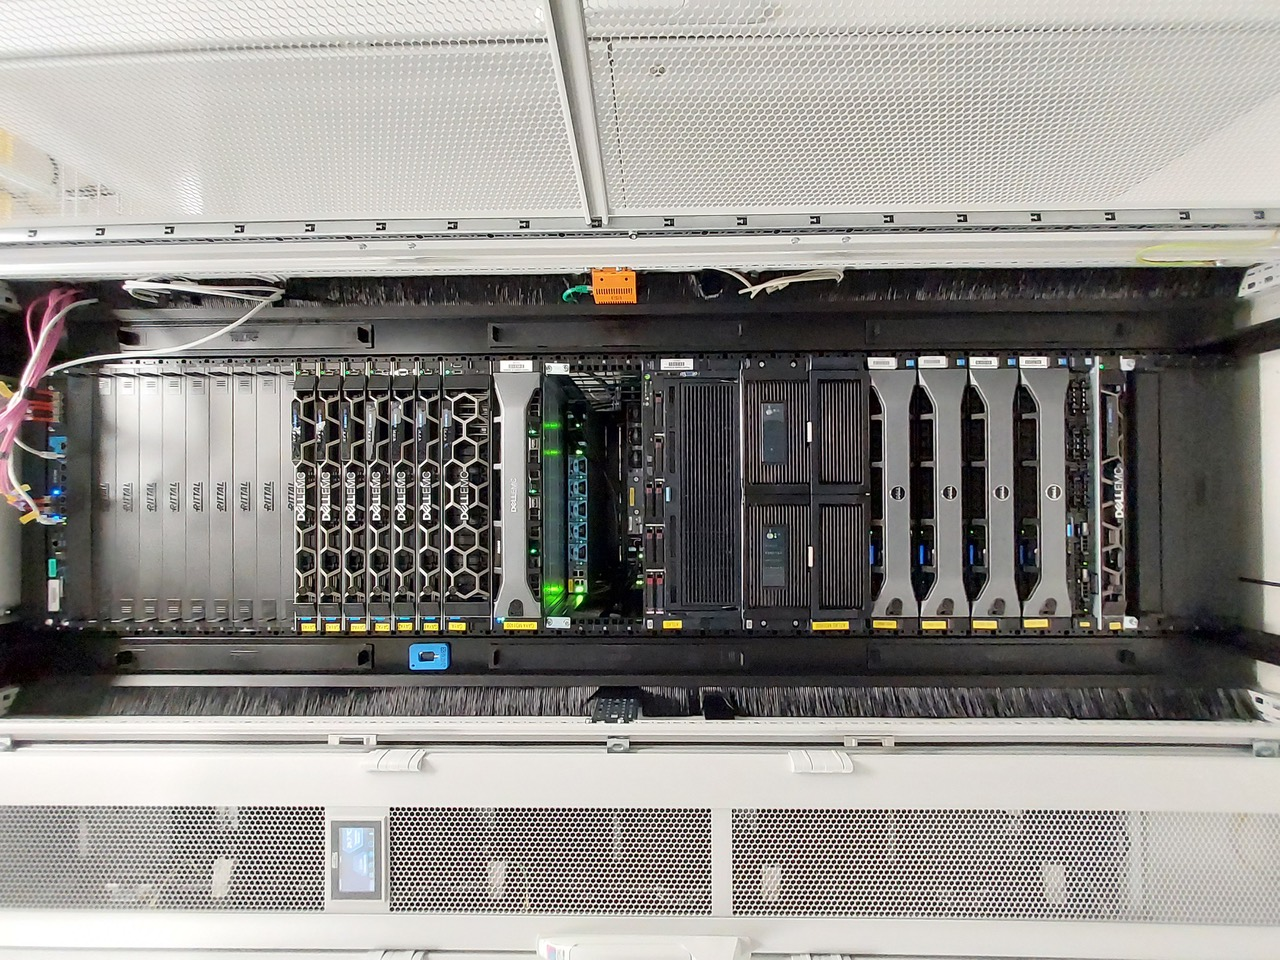
\includegraphics[width=0.7\linewidth, angle=-90]{images/gaya.jpeg}
      \captionof{figure}{Gaya HPC cluster}
    \end{minipage}
    \hfill
    \begin{minipage}{0.49\textwidth}
      \centering
      
\includegraphics[width=0.8\linewidth]{images/git-logo.png}
      \captionof{figure}{Git logo}
    \end{minipage}
  \end{center}
\end{frame}

\section{Possible solutions}
\begin{frame}{Keep the data locally}
  Works but not ideal, especially for:
  \begin{center}
    \begin{minipage}{0.49\textwidth}
      \begin{itemize}
        \item \textbf{Collaboration} (multiple users).
        \item \textbf{Reproducibility} (multiple runs).
        \item \textbf{Continuous integration} (CI).
        \item \textbf{Versioning} (multiple versions).
        \item \textbf{Backup} (multiple copies).
      \end{itemize}
    \end{minipage}
    \hfill
    \begin{minipage}{0.49\textwidth}
      \centering
      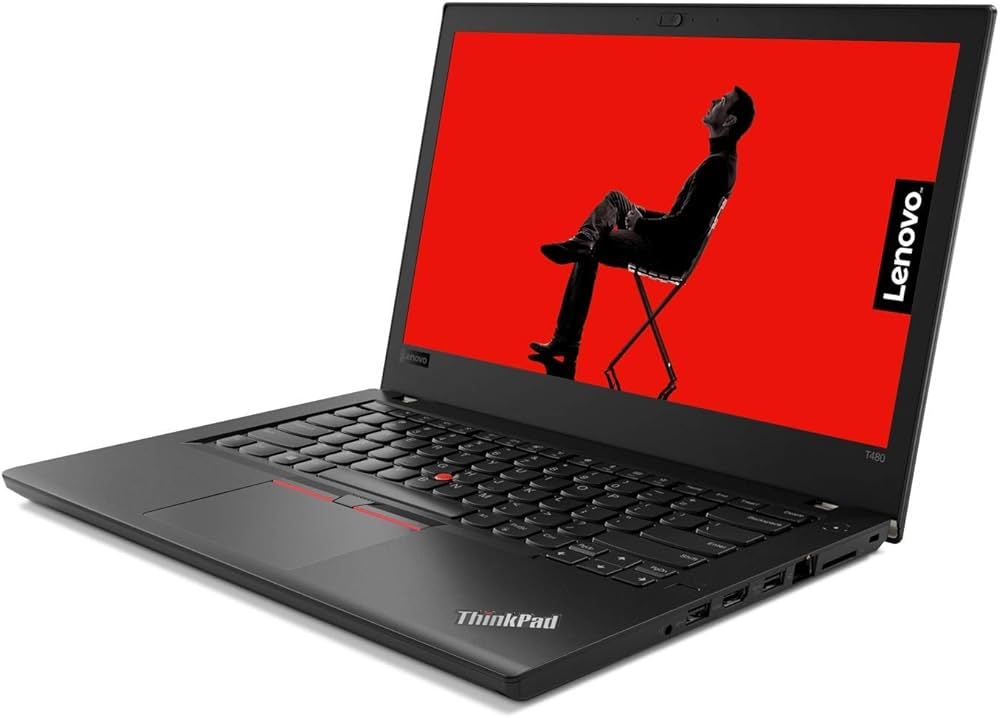
\includegraphics[width=0.6\linewidth]{images/thinkpad.jpg}
      \captionof{figure}{Laptop to keep the data locally}
    \end{minipage}
  \end{center}
\end{frame}

\begin{frame}{Avoidance}
  \begin{minipage}{0.6\textwidth}
    \begin{itemize}
      \item \textbf{File generation} on demand or at execution time.
      \item \textbf{Data reduction:} e.g. only store the most meaningful data.
      \item \textbf{User specifies} which statistics/visualization to generate at each execution.
      \item \textit{etc.}
    \end{itemize}
  \end{minipage}%
  \hfill
  \begin{minipage}{0.4\textwidth}
    \centering
    
\includegraphics[width=\linewidth]{images/avoidance.jpg}
  \end{minipage}
\end{frame}

\begin{frame}{Cloud storage}
  \textbf{For everyday user:} Google Drive, Dropbox, OneDrive, etc.\\
  \textbf{Targeted at scientific collaboration:} Zenodo, Figshare, Dryad, OSF, etc.\\[1ex]
  \begin{minipage}{0.6\textwidth}
    \vspace{0.5cm}
    \textbf{Problematics:}
    \begin{itemize}
      \item \textbf{Requires lots of scripting} to integrate in the HPC workflow.
      \item \textbf{Requires special security measures} to protect sensitive data.
      \item \textbf{How to detect and manage errors?}
      \item \textbf{Compatibility issues}.
    \end{itemize}
  \end{minipage}%
  \hfill
  \begin{minipage}{0.35\textwidth}
    \centering
    
\includegraphics[width=\linewidth]{images/cloud-storage.png}
    % \captionof{figure}{Cloud storage}
  \end{minipage}
\end{frame}

\begin{frame}{Git LFS}
  \begin{minipage}{0.4\textwidth}
    \textbf{Open source extension to Git.}
  \end{minipage}%
  \hfill
  \begin{minipage}{0.6\textwidth}
    
\includegraphics[width=0.8\linewidth]{images/git-lfs-logo.png}
  \end{minipage}

  \vspace{0.5cm}
  \begin{itemize}
    \item Replaces large files with text \textbf{pointers} inside Git, while storing the file contents on a remote server.
    \item \textbf{No need for custom scripting.}
    \item \textbf{Consistent} between local and remote.
  \end{itemize}

  \textbf{Suboptimal usage of local storage:}
  \begin{itemize}
    \item \textbf{Uses locally twice the space} (files are duplicated in \texttt{.git/lfs}).
    \item \textbf{Large files} are \textbf{automatically downloaded} when cloning a repository.
    \item End users have \textbf{nearly no permission/control} on the remote server.
  \end{itemize}
\end{frame}

\begin{frame}{Git-annex}
  \begin{minipage}{0.58\textwidth}
    \textbf{Open source extension to Git.}
    \begin{itemize}
      \item Allows managing large files with Git without checking the file contents into Git.
      \item Uses \textbf{symlinks} to optimize local storage.
      \item \textbf{No duplication} of files.
      \item No intrinsic limit on file size or bandwidth.
    \end{itemize}
    \vspace{0.5cm}
    \textbf{More controls, the user can:}
    \begin{itemize}
      \item decide at anytime which files to keep locally.
      \item use special command to \textbf{download} or \textbf{drop} files.
    \end{itemize}
  \end{minipage}%
  \hfill
  \begin{minipage}{0.38\textwidth}
    \centering
    
\includegraphics[width=\linewidth]{images/git-annex-logo.png}
    % \captionof{figure}{Git-annex logo}
  \end{minipage}
\end{frame}

\begin{frame}{Git-annex}
  Supports the \textbf{download of large files} content from either:
  \begin{itemize}
    \item some \textbf{other git-annex repository} on another machine (if an ssh connection is possible).
    \item a \textbf{cloud storage provider} (e.g. Amazon S3, Google Drive, Dropbox, etc.)
  \end{itemize}
  \vspace{0.5cm}
  \textbf{Main drawback:}
  \begin{itemize}
    \item \textbf{Non natively supported} by GitHub, GitLab, etc. (files needs to be managed with command lines).
    \item \textbf{Learning curve}.
    \item \textbf{Not as common} as Git LFS, support may be harder to find.
  \end{itemize}
\end{frame}

% --------------------------------------
\section{Installation and usage}

\begin{frame}{Installation}
  \begin{center}
    \begin{minipage}{0.2\textwidth}
      \centering
      
\includegraphics[width=0.5\linewidth]{images/Tux.png}
    \end{minipage}%
    \begin{minipage}{0.2\textwidth}
      \centering
      
\includegraphics[width=0.5\linewidth]{images/debian-logo.png}
    \end{minipage}%
    \begin{minipage}{0.2\textwidth}
      \centering
      
\includegraphics[width=0.5\linewidth]{images/archlinux-logo.png}
    \end{minipage}%
    \begin{minipage}{0.2\textwidth}
      \centering
      
\includegraphics[width=0.5\linewidth]{images/macOS-logo.png}
    \end{minipage}
  \end{center}

  \vspace{0.5cm}

  \begin{itemize}
    \item \texttt{sudo apt-get install git-annex} (Debian/Ubuntu)
    \item \texttt{sudo pacman -Syu git-annex} (Arch)
    \item \texttt{brew install git-annex} (MacOS)
  \end{itemize}
\end{frame}

\begin{frame}[fragile]{Usage}
  \textbf{Initialize and add a large file (single quotes are important):}
  \begin{lstlisting}[language=bash]
  git annex init 'PA laptop'
  git annex addurl --file=large_file.zip download_url_link
  # no need to git add
  git commit -m "Add large_file.zip"
  git push origin main git-annex
  git annex list
  git annex whereis large_file.zip
\end{lstlisting}
\end{frame}

\begin{frame}[fragile]{Usage}
  \textbf{Retrieve a file from another repository:}
  \begin{lstlisting}[language=bash]
      git annex init 'Alice laptop'
      git annex get .
    \end{lstlisting}
  \textbf{Annex a newer version:}
    \begin{lstlisting}[language=bash]
      git annex drop large_file.zip
      git rm large_file.zip
      git annex addurl --file=large_file.zip download_url_link
      git commit -m "Update large_file.zip"
      git annex sync
  \end{lstlisting}
\end{frame}

\begin{frame}[fragile]{Usage}
  \textbf{If another user wants to retrieve the newer version:}
  \begin{lstlisting}[language=bash]
    git annex sync
    # Initialize the download :
    git annex get .
  \end{lstlisting}
  \textbf{Check for old orphan symlinks files and their references number:}
  \begin{lstlisting}[language=bash]
    git annex unused
    git annex dropunused NUMBER
    \end{lstlisting}
\end{frame}

\begin{frame}{The end}
  \Large
  \centering
  \textbf{Thank you for your attention!} \\
  \vspace{1em}
  
\includegraphics[height=1cm]{party-emoji.png} \\
  \vspace{1em}
  \textbf{Any questions?} \\
  \vspace{2em}
  \small
  \textit{Contact Information:} \\
  pierre.antoine.senger@gmail.com \\
  github.com/PA-Senger
\end{frame}

\printbibliography


\end{document}
